\subsection{Feuer- und Rauchsimulationen}
Chemischen Reaktionen wie Feuer oder Rauch, der als Volumen, bestehend aus winzigen Partikeln beschrieben werden kann, 
lassen sich nur schwer physikalisch exakt simulieren. Es haben sich hierfür verschiedene Ansätze entwickelt um ein
annähernd realistisches Rendering dieser Phänomene zu erschaffen. Es gibt hierbei zum einen die physikalisch basierten Ansätze. 
Diese beruhen auf aufwändig berechneten Fluidsimulationen und werden vorallem in der Gefahrensimulation verwendet.
Diese sind aufgrund ihrer Komplexität aber nur bedingt echtzeitfähig und werden meist zuvor berechnet. 
Der Fokus liegt dabei meist auf der realistischen Ausbreitung des Feuers und des Rauchs um beispielsweise Fluchtwege 
zu testen oder Evakuierungsszenarien zu simulieren. Diese Anwendungsfälle müssen nicht in Echtzeit berechnet werden.
Daher ist diese Art der Simulation auch für Anwendungen in denen es um die Interaktion mit dem Feuer geht nicht 
effizient nutzbar. Ein Beispiel dafür ist der Einsatz in einem Simulator, der den Umgang mit dem Feuerlöscher
näher bringen soll. Diese basieren zumeist auf effizienteren Partikelsystemen, mit denen sich solche Phänomene 
durch eine Vielzahl an Parametern ebenfalls darstellen lassen. Dieser Ansatz ist jedoch eher von artistischer Natur. 
Zwar lassen sich die Partikel, beispielsweise mit Vektorfeldern, genau steuern, um ein realistisches Aussehen zu 
erzeugen gibt es vorallem in Videospielen andere Methoden, die sich durchgesetzt haben. 


\subsubsection{Feuer}
Feuer, bzw. Flammen sind brennende, Licht und Wärme emittierende Gase, erzeugt durch eine chemische Reaktion. 
\begin{figure}[h!]
	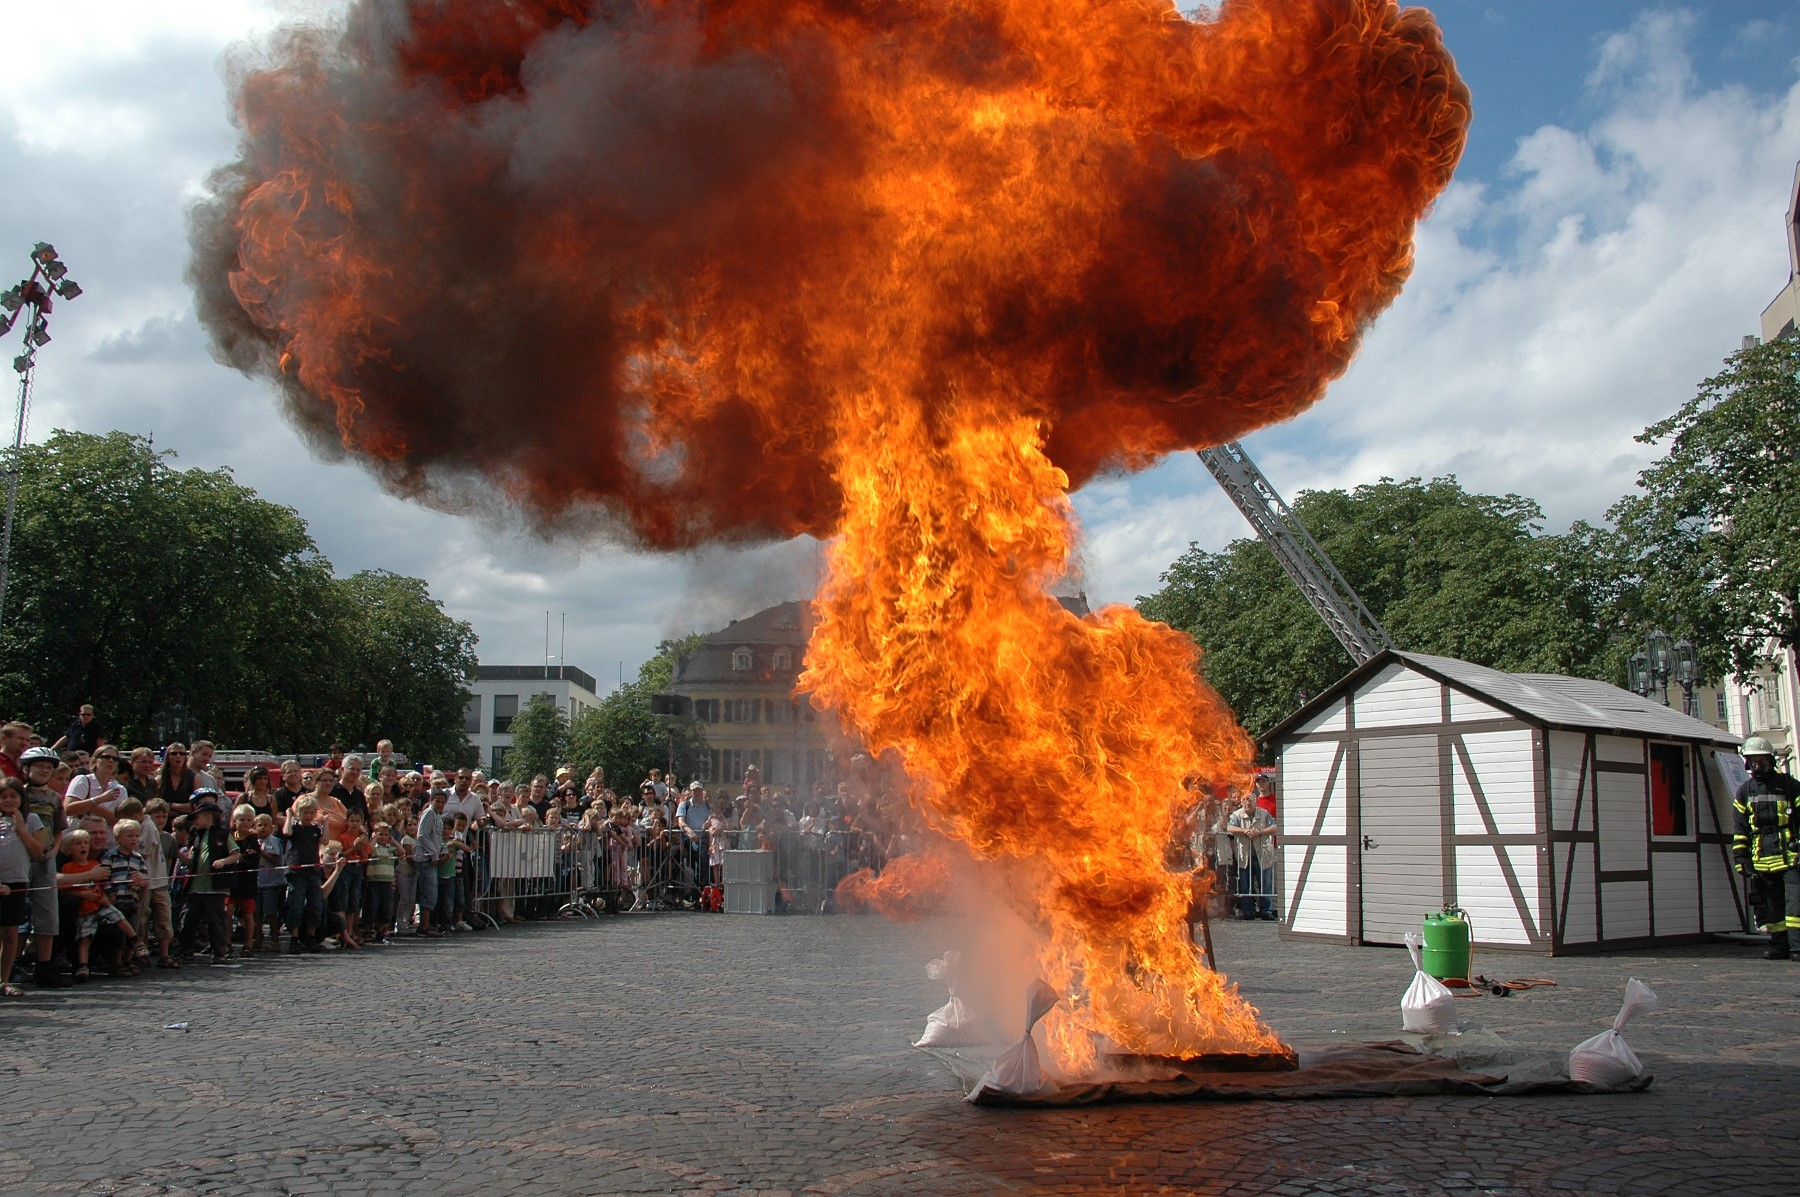
\includegraphics[width=0.89\textwidth]{Grafiken/Basics/Fire/Fettbrand.jpg}
	\centering
	\begin{footnotesize}
		\caption{Fettbrand. Flammen und Rauch mischen sich bei expolosionsartigem Feuer. \\Bild: Der Sascha(\url{https://commons.wikimedia.org/wiki/File:TDFw_135a.jpg}), „TDFw 135a“, \url{https://creativecommons.org/licenses/by-sa/3.0/legalcode}  }

		\label{fig:fettbrand}
	\end{footnotesize}
\end{figure}

<<<<TODO>>>>

\subsubsection{Rauch}
<<<<TODO>>>>

\subsubsection{Partikelsysteme}
<<<<TODO>>>>
